\section{Implementacija}

Implementacija razvijenog modela optimizacije provedena je u programskom jeziku Python, zbog njegove fleksibilnosti, bogatog ekosustava biblioteka te široke primjene u znanstvenom računarstvu i optimizacijskim metodama. Python omogućuje brz razvoj prototipa, jednostavnu integraciju različitih modula te učinkovitu vizualizaciju rezultata.

\subsection{Korištene biblioteke}

Za potrebe izrade sustava korištene su sljedeće biblioteke:
\begin{itemize}
    \item \textbf{NumPy} -- osnovna biblioteka za rad s višedimenzionalnim poljima i vektorima, pruža optimizirane matematičke funkcije te omogućuje učinkovito generiranje slučajnih brojeva potrebnih za Monte Carlo simulacije.
    \item \textbf{random} -- ugrađeni Python modul za generiranje slučajnih vrijednosti, korišten u inicijalnim fazama simulacije i generiranja početnih populacija u genetskom algoritmu.
    \item \textbf{matplotlib} -- biblioteka za vizualizaciju podataka, korištena za grafički prikaz distribucija trajanja zadataka, konvergencije genetskog algoritma i usporedbu dobivenih rješenja.
    \item \textbf{DEAP} (Distributed Evolutionary Algorithms in Python) -- opcionalna biblioteka za implementaciju genetskih algoritama i drugih evolucijskih metoda. Omogućuje jednostavnu definiciju operatora selekcije, križanja i mutacije, kao i prilagodbu parametara evolucijskog procesa.
\end{itemize}

\subsection{Struktura implementacije}

Implementacija je podijeljena u tri glavna modula:
\begin{enumerate}
    \item \textbf{Monte Carlo modul} -- odgovoran za generiranje distribucija trajanja zadataka i procjenu nesigurnosti.
    \item \textbf{Genetski algoritam (GA) modul} -- provodi optimizaciju raspodjele projektnih aktivnosti koristeći rezultate Monte Carlo simulacije.
    \item \textbf{Modul za vizualizaciju} -- omogućuje analizu rezultata kroz grafičke prikaze i usporedbe.
\end{enumerate}

\subsubsection{Monte Carlo modul}

Monte Carlo simulacija implementirana je korištenjem biblioteka \texttt{NumPy} i \texttt{random}. Za svaki zadatak definirana je procijenjena vrijednost trajanja (optimistična, pesimistična i najvjerojatnija procjena). Generiranjem velikog broja simulacija (npr. $10^4$ iteracija), dobivena je empirijska distribucija trajanja svakog zadatka.

Pseudokod implementacije Monte Carlo modula:
\begin{verbatim}
for svaki zadatak u projektu:
    generiraj nasumične vrijednosti trajanja prema odabranoj distribuciji
    spremi rezultate u niz
procijeni prosjek, medijan i standardnu devijaciju trajanja
\end{verbatim}

Rezultat Monte Carlo simulacije je skup distribucija koji se koristi u evaluacijskoj funkciji genetskog algoritma.

\begin{figure}
    \centering
    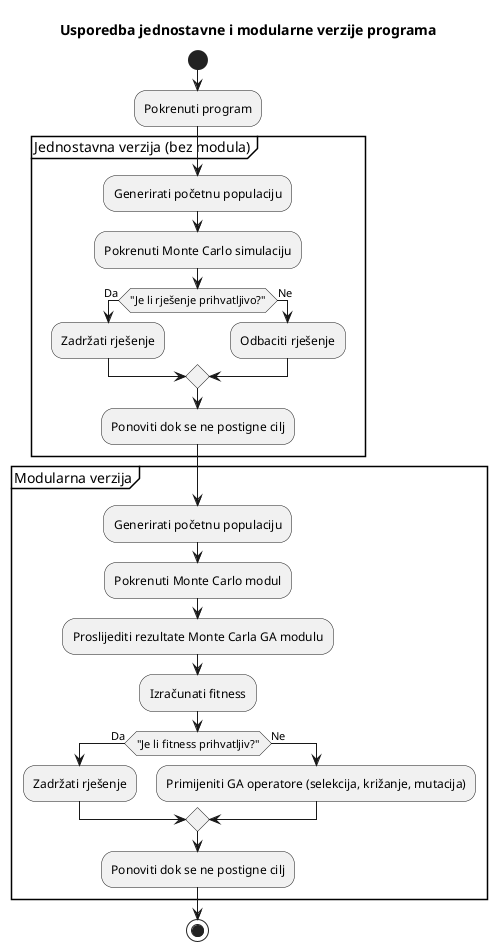
\includegraphics[width=0.9\textwidth]{slike/diagram_mc_ga.png}
    \caption{Dijagram toka procesa optimizacije korištenjem Monte Carlo simulacije i genetskog algoritma}
    \label{fig:diagram_ga_mc}
\end{figure}


\subsubsection{GA modul}

Genetski algoritam implementiran je pomoću biblioteke \texttt{DEAP}, a u slučaju jednostavnije implementacije korišteni su osnovni Python moduli \texttt{random} i \texttt{NumPy}. Ključne komponente GA modula su:
\begin{itemize}
    \item \textbf{Inicijalizacija populacije} -- generira se početna populacija rješenja koja predstavlja različite načine raspodjele projektnih aktivnosti.
    \item \textbf{Funkcija prilagodbe (fitness)} -- izračunava kvalitetu rješenja na temelju trajanja, troškova i vrijednosti dobivenih iz Monte Carlo simulacije.
    \item \textbf{Selekcija} -- odabire najbolja rješenja prema definiranim kriterijima (npr. turnirska selekcija).
    \item \textbf{Križanje (crossover)} -- kombinira dijelove rješenja dvaju roditelja kako bi se stvorila nova, potencijalno bolja rješenja.
    \item \textbf{Mutacija} -- nasumično mijenja dio rješenja radi očuvanja raznolikosti populacije.
    \item \textbf{Zaustavni uvjet} -- algoritam se zaustavlja nakon određenog broja generacija ili kada se konvergencija dostigne.
\end{itemize}

\subsubsection{Vizualizacija rezultata}

Za analizu rezultata korištena je biblioteka \texttt{matplotlib}, a rezultati se prikazuju u tri glavne forme:
\begin{enumerate}
    \item \textbf{Distribucije trajanja zadataka} -- histogrami i krivulje gustoće dobivene iz Monte Carlo simulacija.
    \item \textbf{Konvergencija genetskog algoritma} -- graf promjene najbolje fitness vrijednosti kroz generacije.
    \item \textbf{Usporedba rješenja} -- prikaz najboljeg pronađenog rješenja naspram prosječnih i početnih rješenja.
\end{enumerate}

Ova struktura implementacije omogućuje fleksibilnu nadogradnju sustava, integraciju dodatnih optimizacijskih metoda i prilagodbu različitim vrstama projekata.
